%!TEX root = ../thesis.tex

% https://akhiluk.medium.com/on-why-salvor-hardin-is-simply-the-best-74948711e136
\begin{savequote}[70mm]
	To succeed, planning alone is insufficient.\\One must improvise as well.
	\qauthor{Isaac Asimov, Foundation series}
\end{savequote}

%	Writing a related work section
%	https://www.seas.upenn.edu/~cse400/CSE400_2008_2009/related_work.pdf
%	Your review should: 
%	• Summarize existing research, products and systems 
%	• Talk about trends in the field 
%	• Discuss research themes that emerged from your review 
%	• Place your work in the context of cited work 
%	• Explain why the proposed project is better than or different from what already exists

\chapter{Related work}\label{chapter:related_work}

	Internet  of  Things  is  one  of  the  hottest  topics  in 
	both  industry  and  academia  of  the  communication  engineering 
	world.
	% TODO parlare della rete mesh
	On  the  other  hand,  wireless  mesh  networks,  a  network 
	topology that has been discuss for decades that haven’t been put 
	into use in large scale, can make a difference when it comes to the 
	network  in  the  IoT  world  today.

	This chapter anticipates the one where the actual project is described and shows some related projects from which the open mesh has drawn inspiration.
	
	At first challenges and solutions are presented
	
	Below are also presented some of the projects which have been made at various levels from amateurial projects, to research and to the ones already available on the market.
	
	\section{Challenges and solutions}
		
		% https://beyondroot.com/blog/a-comprehensive-guide-to-mesh-network-in-iot-an-experts-take/
		% Where IoT Mesh Network Can be Usednostro
	
		% https://ieeexplore.ieee.org/document/7968828
		The  single  point  of  failure  nature  of  these  
		Network makes the entire system extremely vulnerable when it 
		comes to disasters or even difficult environment as the sensors 
		may need to be deployed into some hardly reachable locations.
		Besides,  the  capacity  of  the  central  hub/router  of  the  network  
		can  also  limit  the  coverage  of  the  service  provided  by  IoT  
		devices,  and the range is  also constrained by  the  same  factors.
	
		% https://galileodiscovery.unipd.it/discovery/fulldisplay?docid=alma9938985032206046&context=L&vid=39UPD_INST:VU1&lang=it&search_scope=catalogo_no_external&adaptor=Local%20Search%20Engine&tab=Everything&query=any,contains,Wireless%20Mesh%20Networks&offset=0
		Energy management
		
		% https://galileodiscovery.unipd.it/discovery/fulldisplay?docid=alma9938986439606046&context=L&vid=39UPD_INST:VU1&lang=it&search_scope=catalogo_no_external&adaptor=Local%20Search%20Engine&tab=Everything&query=any,contains,Wireless%20Mesh%20Networks&offset=0
	
		% https://ieeexplore.ieee.org/document/4068249
	
	\section{Overview of wireless mesh networks}
	
		% https://haltian.com/resource/top-four-mesh-networks/
	
		% https://www.intechopen.com/chapters/13038
	
		% https://beyondroot.com/blog/a-comprehensive-guide-to-mesh-network-in-iot-an-experts-take/
	
		\subsection{Advantages of WMS}
		
		\subsection{Disasvantages of WMS}
	
	\section{Algorithms for Wireless Mesh networks}
	
						
	
	\section{Projects}
		
		\subsection{Homemade projects}
		
			% https://www.hackster.io/scottpowell69/lora-mesh-chat-5267d9
			
			% https://meshtastic.org/
			% https://github.com/meshtastic
			% https://www.hackster.io/punkgeek/meshtastic-a-hiking-skiing-gps-mesh-communicator-84f999
		
		\subsection{Research projects}
		
			% https://www.springerprofessional.de/en/research-on-using-the-aodv-protocol-for-a-lora-mesh-network/18715992
			
			% BLUETOOTH
			% https://www.ericsson.com/en/reports-and-papers/white-papers/bluetooth-mesh-networking
			
			% https://ieeexplore.ieee.org/document/8071545
			
			\subsubsection{LORACTP}
			
				% https://ieeexplore.ieee.org/document/9394317
			
				\begin{figure}[H]
					\centering
					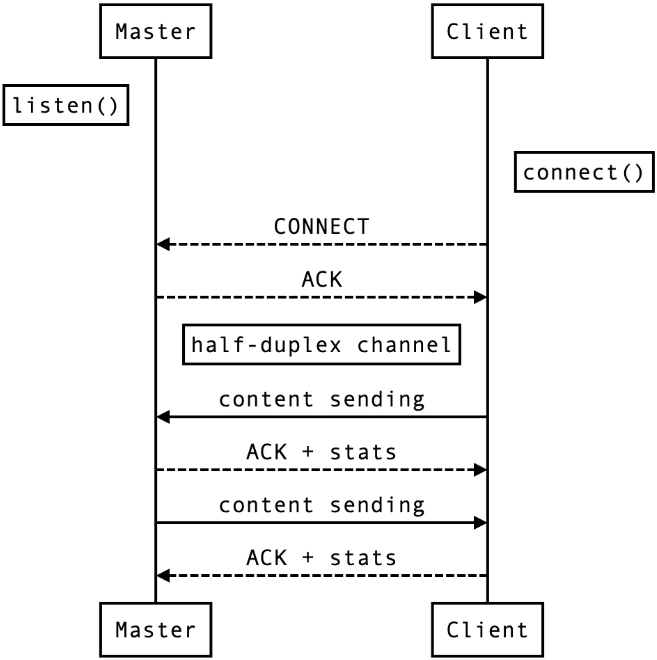
\includegraphics[width=.5\textwidth]{resources/img/loractp_flow}
					\caption{Flow of the establishment and interchange of data in LoRaCTP}
				\end{figure}
		
		\subsection{Market solutions}
		
			% https://www.kickstarter.com/projects/sonnet/sonnet-decentralized-mobile-communication
		
			% https://gotenna.com/
			% https://www.reddit.com/r/RTLSDR/comments/bzian5/ltt_showcases_new_lora_mesh_network_devices/
		
			Pycom itself has an available mesh network that connects lora devices, compared to the one proposed in this paper thought
			% https://docs.pycom.io/pymesh/
			
			% Mesh network in other areas
			% https://www.vmware.com/products/tanzu-service-mesh.html